\documentclass{article}
\usepackage[utf8]{inputenc}
\usepackage{natbib}
\usepackage{graphicx}
\usepackage{lastpage}
\usepackage{xcolor}
\usepackage{lipsum}
\usepackage[T1]{fontenc}
\usepackage{fancyhdr}
\usepackage{geometry}
\usepackage{url}
\usepackage[dutch]{babel}


\usepackage{color}
\usepackage{pdfpages} %om pdf files met requirements lijsten toe te voegen




\bibliographystyle{abbrv} %abbrvnat geeft problemen

\title{Software Requirements Specification}
\author{} %leave empty
\date{} %aanpassen in title_page.tex

\addtolength{\footskip}{1.3cm} % make more space for the footer
\pagestyle{fancyplain} % use fancy for all pages except chapter start
\lhead{}
\cfoot{
\includegraphics[height=1.3cm]{Small_Logo.png}} % right logo
\rfoot{\thepage}
\renewcommand{\headrulewidth}{0.3pt} % remove rule below header
\renewcommand{\footrulewidth}{0.3pt} % remove rule below header

\begin{document}

\makeatletter
\begin{titlepage}

\newcommand{\HRule}{\rule{\linewidth}{0.7mm}} % Defines a new command for the horizontal lines, change thickness here


\vspace*{1.2mm}

\center 

\includegraphics[scale=0.6]{Logo.png}\\[1cm] 
%---------------------------------------------------------------------------------------
%	HEADINGS SECTION
%----------------------------------------------------------------------------------------

\textsc{\LARGE Vrije Universiteit Brussel}\\[0.3cm] % Name of your university/college
\textsc{\large WE-DINF-6537}\\
\textsc{\large Project Software Engineering}\\
\textsc{\large Academiejaar 2014-2015}\\[0.3cm] 
%\textsc{\large Software Engineering}\\[0.7cm] % Major heading such as course name

%----------------------------------------------------------------------------------------
%	TITLE SECTION
%----------------------------------------------------------------------------------------

\HRule \\[0.4cm]
{ \huge \bfseries \@title \\[0.5cm] }
\HRule \\[0.5cm]
 
%----------------------------------------------------------------------------------------
%	AUTHOR SECTION
%----------------------------------------------------------------------------------------

\Large
% laat voorlopig nog even de namen/mailadressen op deze pagina staan
% eerst moeten we zien of er een beter alternatief is om de lege plek dan op te vullen
% anders laten we ze gewoon staan...

%volgens mij ziet het er zo heel goed uit, maar als ze echt wegmoeten mss vub logo groter maken? 
% => OK, ik vind het ook veter zo, we laten ze staan!
Douglas Horemans \textit{<dhoreman@vub.ac.be>}\\
Hannah Pinson \textit{<hpinson@vub.ac.be>}\\
Ivo Vervlimmeren \textit{<ivervlim@vub.ac.be>}\\
Noah Van Es \textit{<noahves@vub.ac.be>}\\
Pieter Steyaert \textit{<psteyaer@vub.ac.be>}\\

\vspace{0.6cm}


\includegraphics[scale=0.4]{VUB_schild.pdf}\\[0.5cm]

{\large 19 november 2014}
\vfill % Fill the rest of the page with whitespace

\end{titlepage}

\newpage
\section*{Versiegeschiedenis}
\addcontentsline{toc}{section}{Versiegeschiedenis}

\begin{center}
\begin{tabular}[t]{| c | c | c | c |}
    \hline
    \textbf{Versie} & \textbf{Datum} & \textbf{Auteurs\cite{note:author}} & \textbf{Beschrijving} \\
    \hline
    
    1.0     &  19/11/2014   &   \begin{tabular}{c} 
                                    Douglas Horemans \\
                                \end{tabular} & Eerste versie \\
    \hline
    2.0     &  15/12/2014   &   \begin{tabular}{c} 
                                    Douglas Horemans \\
                                \end{tabular} & tweede versie \\
    \hline
\end{tabular}
\end{center}
\newpage



\tableofcontents
\newpage

%%%%%%%%%%%%%%%%%%%%%%%%%%%%%%%%%% INTRODUCTIE

\section{Introductie}

%%%
\subsection{Doel en doelpubliek} %van het SRS, niet van het project
Dit is het Software Requirements Specification (SRS) document voor SKRIBL,  een softwareproject uitgevoerd door de groep SE4\_1415 in het kader van het opleidingsonderdeel Software Engineering van de Vrije Universiteit Brussel. Dit document is opgesteld volgens de IEEE 1016-2009 standaard. \newline
\\
\noindent De algemene eisen die de klant aan het op te leveren product stelt zijn te vinden in de projectomschrijving van het opleidingsonderdeel \cite{Xtreport:organisatie}. Dit SRS biedt een globaal, gestructureerd overzicht van deze vereisten (user requirements) in onderdeel (\ref{subsec:userRequirements}). Daarnaast is er een gedetailleerde oplijsting van system requirements die voortvloeien uit deze user requirements, en die dienen als richtlijnen bij het ontwikkelen en testen van het softwareproduct, in onderdeel (\ref{sec:systemRequirements}). In overeenstemming met de principes van een agile development proces worden de system requirements in dit SRS \emph{bij iedere sprint} aangevuld. Meer informatie over het doel en de planning van deze sprints is te vinden in het Software Project Management Plan \cite{Xtreport:SPMP}. \newline
\\
\noindent Dit document is zowel bedoeld voor de klant en externe controle als voor de interne organisatie. In het bijzonder worden de system requirements in onderdeel (\ref{sec:systemRequirements}) door alle leden van het team gebruikt als richtlijnen bij het volledige plannings-, ontwikkelings- en testproces van iedere sprint. De globale oplijsting van requirements in onderdeel (\ref{subsec:userRequirements}) dient als handvest voor de grote lijnen van het software design en de algemene planning van het project.  

%%%
\subsection{Product Scope}
Het doel van dit softwareproject is het ontwikkelen van SKRIBL, een webapplicatie die het enerzijds mogelijk maakt voor onderzoekers om wetenschappelijke publicaties te beheren en die anderzijds de netwerken van deze onderzoekers analyseert en op een aantrekkelijke manier visualiseert. Deze applicatie wordt binnen het kader van het opleidingsonderdeel software engineering gecre\"{e}erd gedurende het academiejaar 2014-2015.

%%%
\subsection{Gebruikte conventies en afkortingen}
Suggesties en opmerkingen voor toekomstige aanpassingen in dit document worden aangeduid met vierkante haakjes en een cursief lettertype: [{\it voorbeeld suggestie}]. \newline
\\
\noindent Volgende afkortingen worden in dit SRS gebruikt:
\begin{itemize}
\item SRS: Software Requirements Specification (document)
\item SPMP: Software Project Management Plan (document)
%\item STD:  Software Test Plan (document)
%\item SDD: Software Design Document (document)
\item FR-U: Functional Requirement, type User
\item FR-P: Functional Requirement, type Publicatie
\item FR-D: Functional Requirement, type Data-Mining
\item NFR-S: Niet-Functionele Requirement, type Security
\item NFR-R: Niet-Functionele Requirement, type Reliability
\item NFR-P: Niet-Functionele Requirement, type Performance
\item G: aangemelde gebruiker
\item B: bezoeker, niet-geauthenticeerde persoon 
\end{itemize}


%%%
\subsection{Referenties}
\begingroup
\renewcommand{\section}[2]{}% verwijdert titel sectie referenties
\bibliography{referenties}
\endgroup

\clearpage
%%%%%%%%%%%%%%%%%%%%%%%%%%%%%%%%%% ALGEMENE BESCHRIJVING 

\section{Algemene Beschrijving}

\subsection{Perspectief van het product}
De ontwikkelde webapplicatie is een op zichzelf staand softwareproduct. Het maakt geen deel uit van andere softwareproducten maar steunt voor een deel van zijn content (i.e., aangeleverde publicaties) op het contacteren van andere websites met gelijkaardige functionaliteiten. \newline
\\
%----comment----%
\noindent [{\it Volgens de IEEE standaard moeten in dit onderdeel verder nog de interfaces (System interfaces; User interfaces; Hardware interfaces; Software interfaces;Communications interfaces) beschreven worden. Indien van toepassing zullen deze onderdelen, in samenspraak met de Software Architect en Configuration Manager, in latere versies aangevuld worden.}]

\subsection{Functies van het product}
\label{subsec:userRequirements}

Hieronder volgt een gestructureerde oplijsting van de functionele vereisten zoals beschreven in de projectomschrijving van het opleidingsonderdeel \cite{Xtreport:organisatie}.

\renewcommand{\labelitemi}{$\diamond$}
\renewcommand{\labelitemii}{$\bullet$}
\renewcommand{\labelitemiii}{$\cdot$}

\begin{itemize}
    %%
    %USER %
    %%
    \item USER
    \begin{itemize}
        \item inloggen en uitloggen 
        \item account aanmaken
        \item account beheren 
        \item aanleggen en beheren van portfolio eigen publicaties
        \item persoonlijke score via portfolio
	\item toevoegen en beheren van lijst publicaties van derden ("favorieten")
	\item publicaties opslaan op eigen computer, buiten applicatie
	\item top drie relevantste publicaties binnen onderzoeksdomein 
	\item suggesties van relevante papers en feed-back/voorkeuren 
	\item opzoeken en toevoegen van publicaties, gevonden in systeem en/of internet, via invulformulier of reeds toegevoegde publicaties
	\item annoteren van publicaties, toevoegen van bijlagen 
	\item publicaties linken op manieren die systeem niet standaard voorziet
	\item raadplegen, genereren en exporteren (PDF) van persoonlijk statistieken en bijhorende grafieken
	\item visualisatie van en interactie met sociaal netwerk in een graaf
	\item mobiele interface
    \end{itemize}
   %%
    %PUBLICATIES %
    %%
    \item PUBLICATIES 
    \begin{itemize}
    \item toevoegen van content + metadata door extractie uit PDF/BibTex en/of manuele aanvulling
    \item weergave van publicaties 
    \item downloaden van het internet
    \item opslaan op computer vd gebruiker (buiten applicatie)
    \end{itemize}
     %%
    %DATAMINING %
    %%
    \item DATAMINING 
    \begin{itemize}
    \item persoonlijke score van gebruiker berekenen adhv portfolio: 
    	\begin{itemize}
    		\item aantal eigen publicaties gedeeld door het aantal maanden sinds de eerste publicatie
   		 \item kwaliteit op basis van de classificatie van conferences en journals
    		\item impact van de eigen publicatie (aantal citaties)
    	\end{itemize}
    \item relevantie van publicatie voor gebruiker berekenen in functie van onderzoeksdomein 
    \item relevantie van publicatie voor gebruiker berekenen op basis van co-auteurs, keywords, ... en dynamische voorkeuren gebruiker 
    \item statistieken voor gebruiker berekenen adhv volgende metrieken (zie ook persoonlijke score)
      	\begin{itemize}
    		\item publicaties per jaar
   		 \item ranking van de publicaties (afhankelijk van de ranking van conference/journal)
    		\item aantal citaties
    	\end{itemize}
    \end{itemize}
\end{itemize}




\subsection{Gebruikers}
De beoogde gebruikers zijn onderzoekers actief in de wetenschappelijke wereld. Deze vormen de enige klasse van gerechtmatigde gebruikers. Daarnaast worden er verschillende veiligheidsmaatregelen ingebouwd om niet-rechtmatige gebruikers de toegang tot de applicatie te ontzeggen. 

\subsection{Omgeving}
Aan de back-end draait het systeem op Wilma, een server beschikbaar gesteld aan de studenten wetenschappen van de Vrije Universiteit Brussel.  Front-end ondersteunt de applicatie alle gangbare en up-to-date browsers. De mobiele interface wordt ontwikkeld voor Android smartphones.

\subsection{Beperkingen op design en implementatie}
JavaScript, HTML5, CSS en bijbehorende open-source frameworks en bibliotheken zijn de enige programmeertalen en technologie\"{e}n die gebruikt mogen worden. In het algemeen mag enkel vrije software aangewend worden, en deze software moet ook verantwoord kunnen worden. Er moet daarnaast ten allen tijde gebruik worden gemaakt van een testing framework. Code moet volgens een vooraf vastgelegde standaard voorzien worden van commentaar. Ten slotte moet GitHub gebruikt worden als (publieke) repository. 

\subsection{Gebruikshandleidingen}

[{\it nog te bepalen}]


\clearpage


%%%%%%%%%%%%%%%%%%%%%%%%%%%%%%%%%% SYSTEEM REQUIREMENTS
\section{Specifieke Requirements}
\label{sec:systemRequirements}

\noindent De functionele requirements zijn opgedeeld in drie types: gebruikers (FR-U), publicaties (FR-P) en data-mining (FR-D); de niet-functionele requirements zijn opgedeeld in de types reliability (NFR-R), performance (NFR-P) en security (NFR-S).  \\
\\
\noindent De hierop volgende secties beschrijven aan de hand van use cases de functionele requirements in detail. Hierbij zijn de prioriteiten niet vermeld, omdat aan sommige onderdelen of varianten van de beschreven scenario's andere prioriteiten toegekend werden. Op het bijgevoegde requirements dashboard kunnen de specifieke prioriteiten afgelezen worden. De prioriteiten worden aangegeven met kleuren en bijhorende lettters:  donkerblauw + H  = hoge prioriteit;  lichtblauw + M = gemiddelde prioriteit;  wit + L = lage prioriteit.


\subsection{Functionele Requirements: USER}
\vspace{4 mm}


%%%%%%%%%%%% REGISTRATIE
\subsubsection{REGISTRATIE}
\vspace{2 mm}

\textbf{ID}: FR-U001
\vspace{2 mm}

\noindent \textbf{Betrokkenen}: bezoeker (B); systeem (S) 
\vspace{2 mm}

\noindent \textbf{Samenvatting}: B voert gewenste account-informatie in. Deze informatie wordt gevalideerd, en NG kan invoer aanpassen waar nodig. Indien alle informatie aan vereisten voldoet wordt een nieuw account geregistreerd. 
\vspace{2 mm}

\noindent \textbf{Pre-conditie}: B bevindt zich op de eerste pagina van de Skribl applicatie. 
\vspace{2 mm}

\noindent \textbf{Trigger}: B geeft aan zich te willen registreren (button)
\vspace{4 mm}

\hrule
\vspace{2 mm}
\noindent \textbf{Scenario}:
\begin{enumerate}
\item B krijgt de mogelijkheid om volgende (verplichte) velden aan te vullen:
\begin{description}
  \item[voornaam en achternaam]  \hfill \\
  {\it moet voldoen aan vereisten voor algemene namen*}
  \item[onderzoeksgroep, departement, faculteit en instelling] \hfill \\
   {\it moet voldoen aan vereisten voor algemene namen*}
  \item[algemene en specifieke onderzoeksdomeinen] \hfill \\
  {\it moet voorkomen in een lijst met algemene en bijhorende specifieke onderzoeksdomeinen}
  \item[username] \hfill \\
    {\it moet uniek zijn; enkel letters, cijfers en underscores toegelaten}
    \item[email] \hfill \\
  {\it moet voldoen aan de standaardvorm voor een e-mailadres.}
       \item[taalvoorkeur] \hfill \\
   {\it NL of EN}
       \item[wachtwoord] \hfill \\
  {\it moet minstens 1 cijfer bevatten; minimum 6 en maximum 20 karakters lang}\\
\end{description}
  \noindent {\it Er mogen geen velden opengelaten worden. *een algemene naam kan accenten, koppeltekens en taal-gebonden speciale karakters bevatten, maar geen cijfers of andere speciale karakters.} 
  
 \item B kan deze informatie doorvoeren (button)  $\hookrightarrow$ A
 \item S controleert en registreert nieuw account  $\hookrightarrow$ B
 \item B krijgt melding van succesvolle registratie 
\end{enumerate}
\noindent \textbf{Alternatief verloop}:
\begin{description}
\item[ $\hookrightarrow$ A] De ingevoerde informatie (uniciteit username wordt niet beschouwd) voldoet niet aan de vereisten. B krijgt een melding en kan informatie aanpassen. $\hookrightarrow$ 1.
\item[ $\hookrightarrow$ B] De ingevoerde username is niet uniek. B krijgt een melding en kan username aanpassen. $\hookrightarrow$ 1.
\end{description}

\vspace{2 mm}
\hrule
\vspace{4 mm}

\noindent \textbf{Post-conditie}: B kan inloggen met eigen username en wachtwoord. \\




%%%%%%%%%%%% LOGIN
\subsubsection{LOGIN}
\vspace{2 mm}

\textbf{ID}: FR-U002
\vspace{2 mm}

\noindent \textbf{Betrokkenen}: bezoeker (B); systeem (S) 
\vspace{2 mm}

\noindent \textbf{Samenvatting}: B vraagt toegang tot de applicatie door invoer van username en wachtwoord. Enkel na invoer van een correcte combinatie wordt de toegang verleend. 
\vspace{2 mm}

\noindent \textbf{Pre-conditie}: B bevindt zich op de eerste pagina van de Skribl applicatie. 
\vspace{2 mm}

\noindent \textbf{Trigger}: B geeft aan zich te willen inloggen (button)

\vspace{4 mm}
\hrule
\vspace{2 mm}
\noindent \textbf{Scenario}:
\begin{enumerate}
\item B krijgt de mogelijkheid om username en wachtwoord in te vullen    
 \item B kan deze informatie doorvoeren (button)
  \item S voert authenticatie uit en verleent toegang voor correcte combinatie username en wachtwoord   $\hookrightarrow$ A
\end{enumerate}
\noindent \textbf{Alternatief verloop}:
\begin{description}
\item[ $\hookrightarrow$ A] De combinatie username / wachtwoord is niet correct. B krijgt een melding en kan informatie aanpassen. $\hookrightarrow$ 1.
\end{description}

\vspace{2 mm}
\hrule
\vspace{4 mm}

\noindent \textbf{Post-conditie}: B is ingelogd en komt op persoonlijk dashboard terecht. \\



%%%%%%%%%%%% LOGOUT
\subsubsection{LOGOUT}
\vspace{2 mm}

\textbf{ID}: FR-U003
\vspace{2 mm}

\noindent \textbf{Betrokkenen}: aangemelde gebruiker (G); systeem (S) 
\vspace{2 mm}

\noindent \textbf{Samenvatting}: G kan op elk moment afmelden.  
\vspace{2 mm}

\noindent \textbf{Pre-conditie}: G is ingelogd. 
\vspace{2 mm}

\noindent \textbf{Trigger}: G geeft aan zich te willen uitloggen (button)

\vspace{4 mm}
\hrule
\vspace{2 mm}
\noindent \textbf{Scenario}:
\begin{enumerate}
  \item S sluit sessie af. 
\end{enumerate}


\vspace{2 mm}
\hrule
\vspace{4 mm}

\noindent \textbf{Post-conditie}: G bevindt zich op de eerste pagina van de Skribl applicatie en is niet meer aangemeld. \\



%%%%%% ACCOUNT VERWIJDEREN 
\subsubsection{ACCOUNT VERWIJDEREN}
\vspace{2 mm}

\textbf{ID}: FR-U004
\vspace{2 mm}

\noindent \textbf{Betrokkenen}: aangemelde gebruiker (G); systeem (S) 
\vspace{2 mm}

\noindent \textbf{Samenvatting}: G kan account verwijderen.  
\vspace{2 mm}

\noindent \textbf{Pre-conditie}: G bevindt zich op dashboard.
\vspace{2 mm}

\noindent \textbf{Trigger}: G geeft aan account te willen verwijderen (button)

\vspace{4 mm}
\hrule
\vspace{2 mm}
\noindent \textbf{Scenario}:
\begin{enumerate}
  \item G krijgt vraag om beslissing te bevestigen 
  \item S verwijdert account 
  \item G krijgt melding van succesvolle verwijdering account
\end{enumerate}


\vspace{2 mm}
\hrule
\vspace{4 mm}

\noindent \textbf{Post-conditie}: G bevindt zich op de eerste pagina van de Skribl applicatie, is niet meer ingelogd en kan voorgaande username en wachtwoord niet meer gebruiken om in te loggen. \\


%%%%%% ACCOUNTGEGEVENS WIJZIGEN

\subsubsection{ACCOUNTGEGEVENS WIJZIGEN}
\vspace{2 mm}

\textbf{ID}: FR-U005
\vspace{2 mm}

\noindent \textbf{Betrokkenen}: aangemelde gebruiker (G); systeem (S) 
\vspace{2 mm}

\noindent \textbf{Samenvatting}: G kan de gegevens van zijn/haar account aanpassen. 
\vspace{2 mm}

\noindent \textbf{Pre-conditie}: G bevindt zich op persoonlijk dashboard.
\vspace{2 mm}

\noindent \textbf{Trigger}: G geeft aan accountgegevens te willen wijzigen (button)

\vspace{4 mm}
\hrule
\vspace{2 mm}
\noindent \textbf{Scenario}:
\noindent Dit scenario is analoog aan het scenario REGISTRATIE. De velden zijn in dit geval ingevuld met reeds aanwezige accountgegevens; de username van een gebruiker kan niet gewijzigd worden. 

\vspace{2 mm}
\hrule
\vspace{4 mm}

\noindent \textbf{Post-conditie}: G krijgt een melding van succesvolle aanpassing. \\



%%%%%% TAALKEUZE

\subsubsection{TAALKEUZE}
\vspace{2 mm}

\textbf{ID}: FR-U006
\vspace{2 mm}

\noindent \textbf{Betrokkenen}: bezoeker (B) of aangemelde gebruiker (G); systeem (S) 
\vspace{2 mm}

\noindent \textbf{Samenvatting}: De interface kan in twee talen, Engels en Nederlands, aangeboden worden. 
\vspace{2 mm}

\noindent \textbf{Pre-conditie}: Indien G, dan wordt de interface aangeboden volgens de taalvoorkeur van de gebruiker, meegegeven bij registratie.
\vspace{2 mm}

\noindent \textbf{Trigger}: G/B geeft aan de taal te willen wijzigen naar Engels of Nederlands (button)

\vspace{4 mm}
\hrule
\vspace{2 mm}
\noindent \textbf{Scenario}:
\noindent S laadt een nieuwe interface waarin de taal aangepast is.
\vspace{2 mm}
\hrule
\vspace{4 mm}

\noindent \textbf{Post-conditie}: G/B ziet een interface in de door hem/haar gekozen taal. \\




%%%%%% 

\subsubsection{AUTEURSNETWERK}
\vspace{2 mm}

\textbf{ID}: FR-U007(+)
\vspace{2 mm}

\noindent \textbf{Betrokkenen}: aangemelde gebruiker (G); systeem (S) 
\vspace{2 mm}

\noindent \textbf{Samenvatting}: Een gebruiker kan netwerken van co-auteurs raadplegen in een interactieve graaf. 
\vspace{2 mm}

\noindent \textbf{Pre-conditie}: G is aangemeld en bevindt zich op het dashboard.
\vspace{2 mm}

\noindent \textbf{Trigger}: G geeft aan zijn/haar netwerk te willen weergeven. 

\vspace{4 mm}
\hrule
\vspace{2 mm}
\noindent \textbf{Scenario}:
\begin{enumerate}
\item S genereert een graaf van co-auteurs aan de hand van informatie in de database
\item Aan de hand van kleurcodes en visuele elementen worden in de graaf Skribl gebruikers van andere auteurs onderscheiden, en kan de relatieve impact van auteurs (i.e., tov de huidige gebruiker) ge\"inspecteerd worden. 
\item G krijgt na het klikken op een node in de graaf basisinformatie over de aangeklikte auteur te zien. G kan vervolgens ook zijn/haar netwerk laten genereren.
\item G krijgt na het klikken op een link een lijst van publicaties te zien, horende bij de link die twee auteurs verbindt. G kan (de metadata van) deze publicaties bekijken, en deze eventueel toevoegen aan zijn/haar bibliotheken. 
\end{enumerate}
\vspace{2 mm}
\hrule
\vspace{4 mm}

\noindent \textbf{Post-conditie}: /. \\






\clearpage


%%%%%%%%%%%%%%%%PUBLICATIE%%%%%%%%%%%%%%%%%%%%


\subsection{Functionele Requirements: PUBLICATIE}
\vspace{4 mm}

%%%%%%%%%%%% PUBLICATIE UPLOADEN 
\subsubsection{PUBLICATIE UPLOADEN}
\vspace{2 mm}

\textbf{ID}: FR-P001
\vspace{2 mm}

\noindent \textbf{Betrokkenen}: aangemelde gebruiker (G); systeem (S) 
\vspace{2 mm}

\noindent \textbf{Samenvatting}: G kan een bestand uploaden in PDF- of Bibtex-formaat, waarna S metadata uit dit bestand extraheert; de gevonden metadata kan manueel aangevuld worden door de gebruiker. Het bestand en metadata worden opgeslagen door S. 
\vspace{2 mm}

\noindent \textbf{Pre-conditie}: G bevindt zich op persoonlijk dashboard.  
\vspace{2 mm}

\noindent \textbf{Trigger}: G geeft aan een publicatie te willen uploaden (button)
\vspace{4 mm}



\hrule
\vspace{2 mm}
\noindent \textbf{Scenario}:
\begin{enumerate}
\item G geeft de titel en het type van de publicatie in 
\item S controleert of publicatie met die titel reeds aanwezig is.  $\hookrightarrow$ A
\item G krijgt de mogelijkheid om bestand uit eigen filesystem toe te voegen.
\item S controleert of bestand PDF formaat heeft $\hookrightarrow$ B
\item S vult waar mogelijk volgende metadata aan:
\begin{description}
  \item[titel (V)]  \hfill 
  \item[auteurs (V) ] \hfill 
  \item[indien journal: naam/volume/nummer (V)] \hfill 
  \item[indien proceeding: naam/organisatie (V)] \hfill 
  \item[jaar van publicatie (V) ] \hfill 
  \item[onderzoeksdomein (V)]  \hfill 
  \item[keywords]  \hfill 
  \item[abstract] \hfill 
   \item[aantal citaties] \hfill 
    \item[URL] \hfill 
  \end{description}
\item S controleert of de door scraping gevonden auteurs reeds aanwezig zijn in het systeem. 
\item G kan deze metadata verder aanvullen of wijzigen, en kan oordelen of de in het systeem gevonden auteurs de gewenste auteurs zijn (adhv publicaties van de gevonden auteurs) 
 \item G kan deze informatie doorvoeren (button)  $\hookrightarrow$ C
 \item S slaat publicatie op   
 \item B krijgt melding van succesvol toevoegen publicatie 
\end{enumerate}
\noindent \textbf{Alternatief verloop}:
\begin{description}
\item[ $\hookrightarrow$ A] Een publicatie met dezelfde titel is reeds aanwezig in het systeem. G oordeelt of het over dezelfde publicatie gaar, indien ja, dan wordt deze publicatie aan de bibliotheek van de gebruiker toegevoegd. 
\item[ $\hookrightarrow$ B] Het bestand heeft niet het juiste formaat. G krijgt een melding. $\hookrightarrow$ 1.
\item[ $\hookrightarrow$ C] De ingevoerde metadata voldoet niet aan de validatie-vereisten. G krijgt een melding en kan aanpassingen doorvoeren. $\hookrightarrow$ 5.
\end{description}

\vspace{2 mm}
\hrule
\vspace{4 mm}


\noindent \textbf{Post-conditie}: Een nieuwe publicatie met bijhorende metadata is opgeslagen in  de bibliotheek van de gebruiker. \\



%%%%%%%%%%%% OPZOEKEN EN BEWAREN VAN PUBLICATIE
\subsubsection{OPZOEKEN EN BEWAREN VAN PUBLICATIE}
\vspace{2 mm}

\textbf{ID}: FR-P002
\vspace{2 mm}

\noindent \textbf{Betrokkenen}: aangemelde gebruiker (G); systeem (S) 
\vspace{2 mm}

\noindent \textbf{Samenvatting}: G kan zoeken naar een publicatie op twee verschillende manieren: door het invoeren van een generieke zoekterm (=basic search), waarna resultaten verzameld worden zowel in het Skribl systeem als via google scholar; of via een uitgebreide zoekopdracht, waarna publicaties enkel gezocht worden binnen het Skribl systeem. G kan de gevonden publicaties toevoegen aan zijn/haar gekozen bibliotheek. 
\vspace{2 mm}

\noindent \textbf{Pre-conditie}: G bevindt zich in bibliotheek. 
\vspace{2 mm}

\noindent \textbf{Trigger}: G geeft aan publicaties te willen zoeken (form en button)
\vspace{4 mm}

\hrule
\vspace{2 mm}
\noindent \textbf{Scenario}:
\begin{enumerate}
\item G vult een generieke zoekterm in, of geeft aan een uitgebreide zoekopdracht te willen uitvoeren met als mogelijke parameters titel, jaar, keywords en auteurs.
\item G klikt aan de zoekopdracht te willen uitvoeren (button)
\item S doorzoekt eigen systeem van openbare publicaties en verzamelt relevante publicaties
\item indien basis zoekopdracht, dan contacteert S Google Scholar en verzamelt relevante publicaties
\item G ziet een lijst van de gevonden publicaties en kan de metadata (inclusief abstract, indien aanwezig) inspecteren
\item G kan de PDF openen of de URL naar de gevonden PDF openen 
\item G kan ervoor kiezen de publicatie (PDF/URL + metadata) in zijn bibliotheek of portfolio op te slaan
\end{enumerate}

\vspace{2 mm}
\hrule
\vspace{4 mm}

\noindent \textbf{Post-conditie}: Een nieuw bestand (PDF of URL) met bijhorende metadata is opgeslagen in het systeem / de bibliotheek van de gebruiker. \\


\subsubsection{BIBLIOTHEEK}
\vspace{2 mm}

\textbf{ID}: FR-P003
\vspace{2 mm}

\noindent \textbf{Betrokkenen}: aangemelde gebruiker (G); systeem (S) 
\vspace{2 mm}

\noindent \textbf{Samenvatting}: G kan publicaties toevoegen en beheren in 'bibliotheken'. De standaard bibliotheken zijn: alle bewaarde publicaties, een portfolio (bestaande uit eigen publicaties), en favorieten (bestaande uit bewaarde publicaties van derden). G kan hier bliotheken aan toevoegen. 
\vspace{2 mm}

\noindent \textbf{Pre-conditie}: G bevindt zich in bibliotheek. 
\vspace{2 mm}

\noindent \textbf{Trigger}: / 
\vspace{4 mm}

\hrule
\vspace{2 mm}
\noindent \textbf{Scenario}:
\begin{enumerate}
\item portfolio: G kan een lijst van eigen publicaties beheren 
\item favorieten: G kan een lijst van andere publicaties beheren 
\item alle bewaarde publicaties: G kan een lijst van al zijn bewaarde publicaties (portfolio + favorieten) beheren 
\item G kan een nieuwe bibliotheek aanmaken
\item G kan in elk van deze bibliotheken een publicatie toevoegen, via een zoekopdracht of vanuit het eigen systeem 
\item G kan in elk van deze bibliotheken een publicatie verwijderen 
\item G kan aangeven dat een publicatie privaat is 
\item G krijgt na selectie van een publicatie de metadata van deze publicatie te zien
\item G kan de PDF openen of kan de link naar de PDF volgen 
\end{enumerate}

\vspace{2 mm}
\hrule
\vspace{4 mm}


\noindent \textbf{Post-conditie}: / \\


\subsubsection{PDF-VIEWER}
\vspace{2 mm}

\textbf{ID}: FR-P004
\vspace{2 mm}

\noindent \textbf{Betrokkenen}: aangemelde gebruiker (G); systeem (S) 
\vspace{2 mm}

\noindent \textbf{Samenvatting}: G kan publicaties bekijken met behulp van een ingebouwde PDF viewer. \vspace{2 mm}

\noindent \textbf{Pre-conditie}: G is aangemeld 
\vspace{2 mm}

\noindent \textbf{Trigger}: G klikt op een publicatie die hij/zij wil bekijken 
\vspace{4 mm}

\hrule
\vspace{2 mm}
\noindent \textbf{Scenario}:
\begin{enumerate}
\item  G kan de publicatie bekijken in een viewer
\item G kan inzoomen, uitzoomen en door het document bladeren 
\end{enumerate}
\vspace{2 mm}
\hrule
\vspace{4 mm}


\noindent \textbf{Post-conditie}: / \\




\clearpage


%%%%%%%%%%%%%%%%DATA -MINING%%%%%%%%%%%%%%%%%%%%


\subsection{Functionele Requirements: DATA-MINING}
\vspace{4 mm}


\subsubsection{GOOGLE SCHOLAR SCRAPING}
\vspace{2 mm}

\textbf{ID}: FR-D001
\vspace{2 mm}

\noindent \textbf{Betrokkenen}: systeem (S), Google Scholar (GS)
\vspace{2 mm}

\noindent \textbf{Samenvatting}: S kan gegevens en metadata verzamelen via http requests naar Google Scholar  
\vspace{2 mm}

\noindent \textbf{Pre-conditie}: /
\vspace{2 mm}

\noindent \textbf{Trigger}: Gebruiker voegt nieuwe paper toe en wil metadata opvragen, gebruiker voert zoekopdracht uit, etc.
\vspace{4 mm}

\hrule
\vspace{2 mm}
\noindent \textbf{Scenario}:
\begin{enumerate}
\item S kan volgende, mogelijk onvolledige, metadata verzamelen via een one-form GS zoekopdracht 
\begin{description}
  \item[titel]  \hfill
  \item[auteurs] \hfill 
   \item[abstract] \hfill
   \item[titel van journal of proceedings ] \hfill 
    \item[uitgever] \hfill 
   \item[jaar van publicatie] \hfill 
    \item[aantal citaties] \hfill
   \item[URL] \hfill 
  \end{description}
\end{enumerate}

\vspace{2 mm}
\hrule
\vspace{4 mm}


\noindent \textbf{Post-conditie}: / \\



\subsubsection{SUGGESTIES}
\vspace{2 mm}

\textbf{ID}: FR-D002
\vspace{2 mm}

\noindent \textbf{Betrokkenen}: systeem (S), Gebruiker (G)
\vspace{2 mm}

\noindent \textbf{Samenvatting}: G kan een eenvoudige rating aan publicaties toekennen. S kan vervolgens op basis van deze gegevens nieuwe publicaties aan G voorstellen. 
\vspace{2 mm}

\noindent \textbf{Pre-conditie}: /
\vspace{2 mm}

\noindent \textbf{Trigger}: Gebruiker opent 'recommendations' view.
\vspace{4 mm}

\hrule
\vspace{2 mm}
\noindent \textbf{Scenario}:
\begin{enumerate}
\item G ziet een lijst van voorgestelde publicaties.
\item G kan deze publicaties bekijken, toevoegen aan zijn/haar bibliotheken, alsook een 'like' of 'dislike' aan deze publicaties toekennen. 
\item S kan aan de hand van de rating en de bijhorende metadata van de publicatie nieuwe publicaties voorstellen aan de gebruiker. 
\end{enumerate}
\noindent \textbf{Post-conditie}: / \\










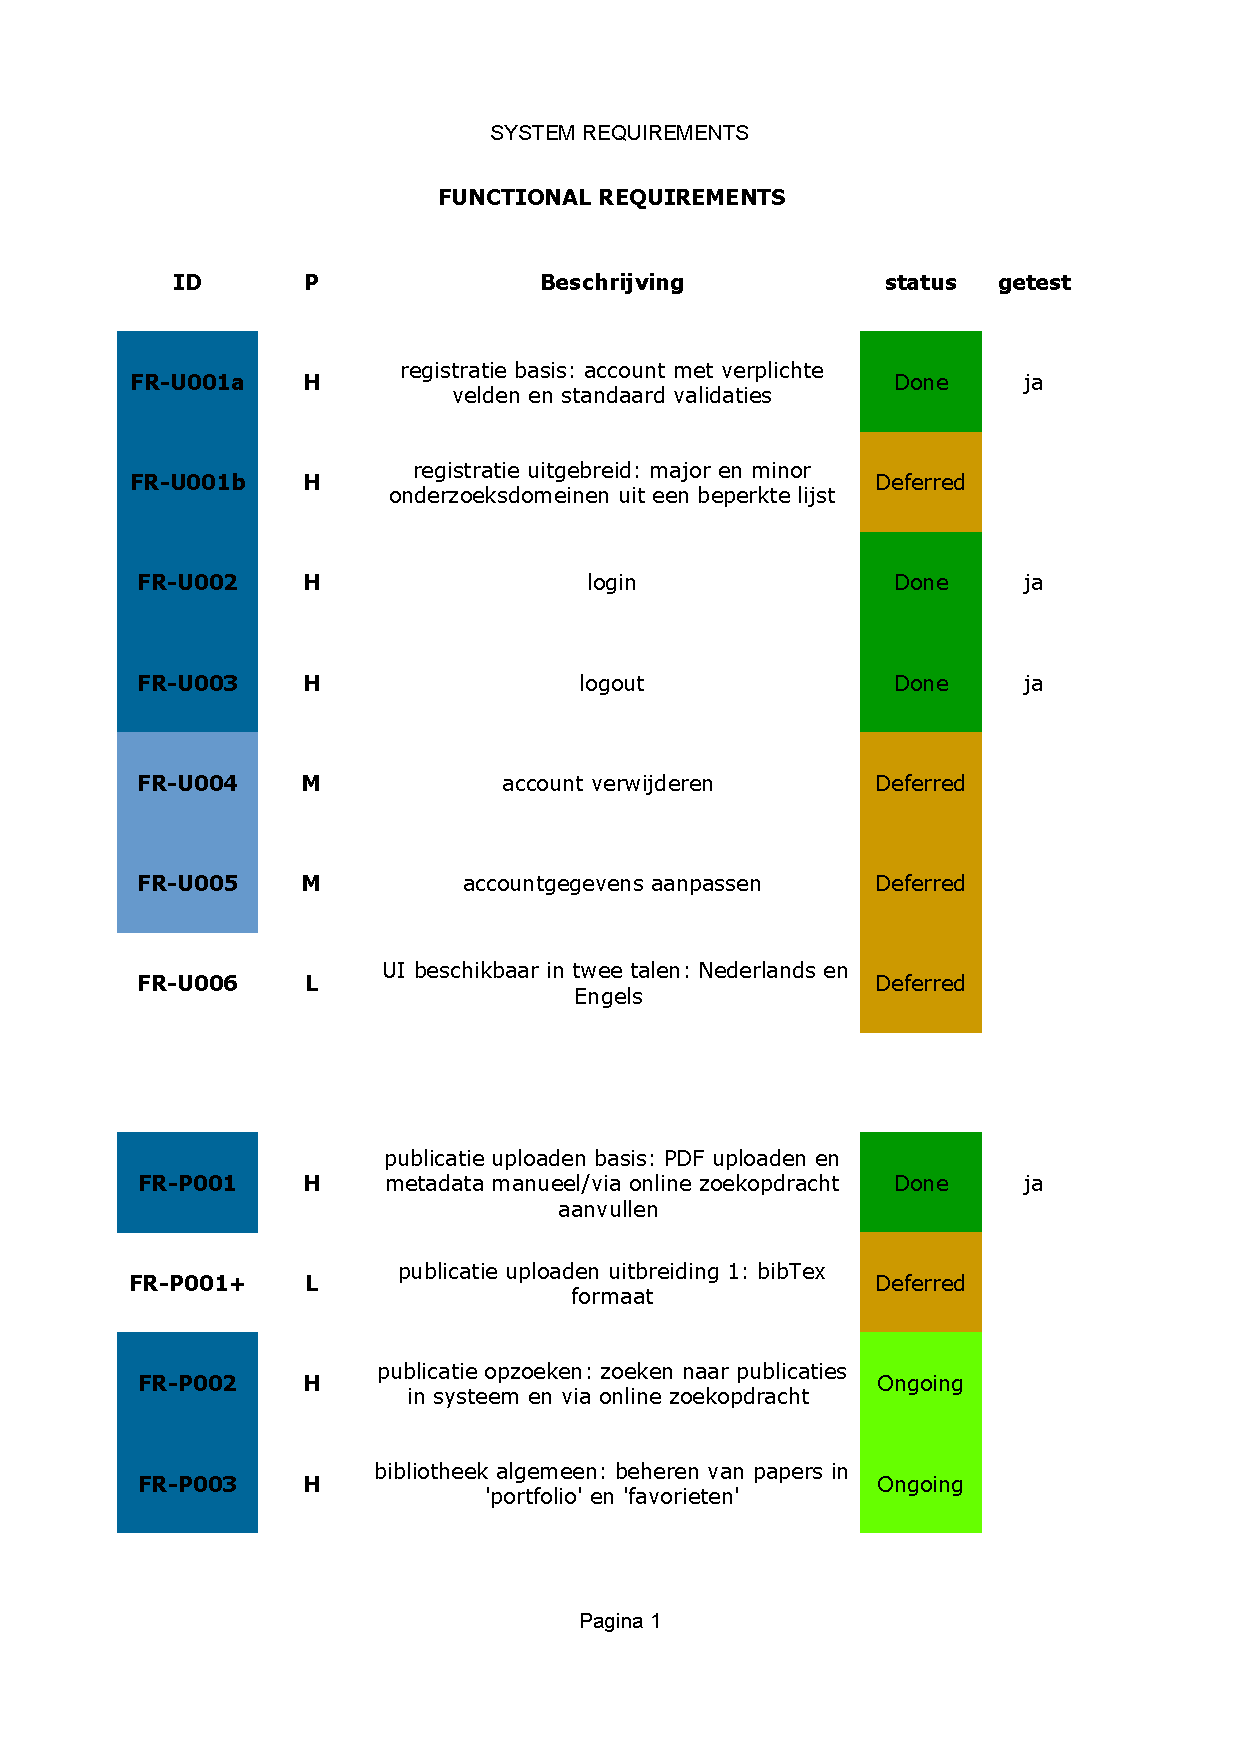
\includepdf[pages={-}]{requirements_dashboard_2maart.pdf}








\end{document}
